\chapter{Detecting Political Bias In News Content} \label{chap:ensemble-bert}

\todo{emphasise within news}

In this chapter we survey existing models to detect political bias, using the News-Media-Reliability dataset \cite{news-media-reliability}. Baly et al. already provide an SVM classifier that uses the News-Media-Reliability pre-computed features to detect bias (see Section \ref{subsec:svms}). We compare this to other popular classifiers used in literature, as well as ensemble classifiers that have not been explored previously in detail (Section \ref{sec:nmr-ensemble}). We then assemble our own dataset of raw article text, and explore using features learned automatically from the text with BERT (Section \ref{sec:nmr-bert}).

\section{Using ensemble classifiers} \label{sec:nmr-ensemble}

The pre-computed features in the News-Media-Reliability dataset include feature vectors based off article text, Twitter pages, Wikipedia pages and web traffic (see Section \ref{subsec:news-media-reliability} for more details about the dataset). In an ablation study, Baly et al. found that the features extracted from the actual article content provided the best classifier performance, however the Wikipedia, Twitter and web traffic features were not very useful for predicting bias. This intuitively makes sense, as not much extra information about bias can be derived from the Wikipedia or Twitter content of the news source. We therefore don't consider individual Twitter, Wikipedia and web traffic features in our results - we simply compare the performance using all pre-computed features vs only article text features.

\subsection{Data pre-processing}

The News-Media-Reliability features we use are already provided in numerical vector format, so no additional pre-processing needs to be done here. However, there is significant class imbalance among the 7 labels used in the data.

The original labels are \textit{extreme-left, left, center-left, center, center-right, right} and \textit{extreme-right}. We merge \textit{extreme-left} and \textit{extreme-right} into \textit{left} and \textit{right} respectively, due to \textit{extreme-left} being very small in size. We also remove the \textit{left-center} and \textit{right-center} classes, since \textit{right-center} is small in size, and these are ambiguous transitionary classes that can't necessarily be merged into \textit{center} or \textit{left/right}. Table \ref{tab:nmr-class-balancing} shows the class sizes before and after pre-processing.

\begin{table}[h]
    \begin{center}
        \begin{tabular}{|c|c|c|c|c|c|c|}
            \hline
            extreme-left & left & left-center & center & right-center & right & extreme-right \\
            \hline
            21 & 168 & 209 & 263 & 92 & 157 & 156 \\
            \hline
        \end{tabular}
    \end{center} \vspace{5pt}
    \begin{center}
        \begin{tabular}{|c|c|c|}
            \hline
            left & center & right \\
            \hline
            189 & 263 & 313 \\
            \hline
        \end{tabular}
    \end{center}
    \caption{News-Media-Reliability original classes (top) vs. final classes used (bottom)}
    \label{tab:nmr-class-balancing}
\end{table}

There is still some class imbalance between left and right, however the overall imbalance has been greatly reduced.

\subsection{Evaluation}

We compare six classifiers in total: 3 non-ensemble methods (SVMs, multi-layer perceptrons and decision trees) and 3 ensemble methods (random forests, Adaboost and gradient-boosted forests). Random forests are of course an ensemble of decision trees, and Adaboost and gradient-boosted forests both implement different gradient-boosting algorithms.

For each experiment we use 5-fold cross validation, and within each fold we use an 80:20 train/test split. All classifiers are implemented using the Python \texttt{scikit-learn} package \cite{sklearn}, using the \texttt{GridSearchCV} method for hyperparameter tuning.

Results are shown in Table \ref{tab:nmr-ensemble-results}, given to 2 decimal places. The highest performing classifier for each metric is highlighted in \textbf{bold}. We report macro-averaged F1 score, accuracy, mean absolute error (MAE) and macro-averaged mean absolute error ($ MAE^M $). $ MAE^M $ is a weighted average of errors for each class, where the weights are inversely proportional to the size of each class i.e. smaller classes' errors are upweighted more. This metric is much more robust to class imbalance than MAE.

\begin{table}[h]
    \centering
    \small
    \begin{adjustbox}{width=1.1\textwidth,center}
    \begin{tabular}{|c|c|c|c|c|c|c|c|c|c|}
        \hline
        \textbf{Classifier} & \multicolumn{4}{|c|}{\textbf{All features}} & \multicolumn{4}{|c|}{\textbf{Only text-based features}} \\
         & \textbf{Macro-F1} & \textbf{Acc.} & \textbf{MAE} & $ \textrm{\textbf{MAE}}^M $ & \textbf{Macro-F1} & \textbf{Acc.} & \textbf{MAE} & $ \textrm{\textbf{MAE}}^M $ \\
         \hline
         SVM & \textbf{67.07} & \textbf{68.76} & 0.46 & 0.50 & 64.93 & 66.27 & 0.45 & 0.48  \\
         MLP & 54.90 & 60.26 & 0.56 & 0.66 & 58.17 & 61.57 & 0.52 & 0.59 \\
         Decision tree & 48.28 & 49.80 & 0.67 & 0.70 & 49.03 & 49.80 & 0.70 & 0.71 \\
         \hline
         Random forest & 59.52 & 64.71 & 0.49 & 0.57 & 57.95 & 63.53 & 0.51 & 0.60 \\
         Adaboost & 59.04 & 62.48 & 0.53 & 0.61 & 59.23 & 61.44 & 0.54 & 0.59 \\
         Grad-boosted forest & 66.17 & 68.10 & \textbf{0.44} & \textbf{0.48} & \textbf{65.85} & \textbf{67.45} & \textbf{0.44} & \textbf{0.48} \\
         \hline
    \end{tabular}
    \end{adjustbox}
    \caption{Bias detection results using pre-computed features across different classifiers}
    \label{tab:nmr-ensemble-results}
\end{table}

We see that using all features, the highest performing classifiers is the SVM, with gradient-boosted forests coming in a close second. Only using the text-based features, gradient-boosted trees perform the best. Hence ensemble classifiers do show a small improvement ($ \approx $ 1\%) over the other, weaker learners for this particular problem.


Baly et al. report an SVM macro-F1 score of 61.31\% and accuracy of 68.86\%. Our SVM manages to achieve a similar accuracy, however our macro-F1 score is around 6 percentage points higher. This could be attributed to our differences in dealing with class imbalance - Baly et al. merge \textit{center-left} and \textit{center-right} into the \textit{center} class, whereas we actually remove the transitionary classes altogether. Our higher F1 score could signify that keeping a distinct boundary between left-wing and right-wing content improves classifier performance, even if the amount of training data available is reduced. Merging \textit{left-center} and \textit{right-center} into the \textit{center} class may confuse the classifier, causing it to mispredict.

We note for all classifiers except for MLPs, the accuracy and F1-scores are higher using all the features vs only text-based features, however the difference is within around 2 percentage points. This backs up the claims by Baly et al., who report that the non-textual features do not provide much additional information to the model.

The best hyperparameters for our SVM were RBF as the kernel function, degree of polynomial decision boundary = 3, $ C = 100 $ and $ \gamma = 0.001 $. The best gradient-boosted forest hyperparameters were: no. estimators = 100, learning rate = 0.6 and minimum samples in a leaf node = 5.

\section{Using BERT} \label{sec:nmr-bert}

Whereas the previous ensemble classifiers take in manually engineered features, BERT models learn the optimal features straight from the raw text. We therefore create our own dataset of news article text (including headline and article body text). These were scraped from the web using an open source tool called \texttt{NewsScraper} \cite{newsscraper}, which is based off of the Python \texttt{newspaper} \cite{newspaper-python} package.

We scrape from all news sources present in the News-Media-Reliability dataset. After class merging from Section \ref{sec:nmr-ensemble} we have 732 sources to consider. Many of these sources use front-end code formats NewsScraper cannot parse - NewsScraper only managed to scrape articles from 432 of these news sources. We collect a maximum of 5 articles per news source, giving us a total of 1654 news articles (note that not all news sites had 5 available articles to scrape). For each article we store the article headline, article body text, and the political bias label for this news source as given by Media Bias/Fact Check (\textit{left}, \textit{center} or \textit{right}). A portion of the dataset is shown in Figure \ref{fig:nmr-bert-data}. The distribution of classes is shown in Table \ref{tab:nmr-bert-data-classes} - there are a significant amount more right-wing articles than center or left articles.

\begin{table}[h]
    \centering
    \begin{tabular}{|c|c|c|}
        \hline
        left & center & right \\
        \hline
        430 & 567 & 657 \\
        \hline
    \end{tabular}
    \caption{Class distribution in self-assembled article text dataset}
    \label{tab:nmr-bert-data-classes}
\end{table}

\begin{figure}
    \centering
    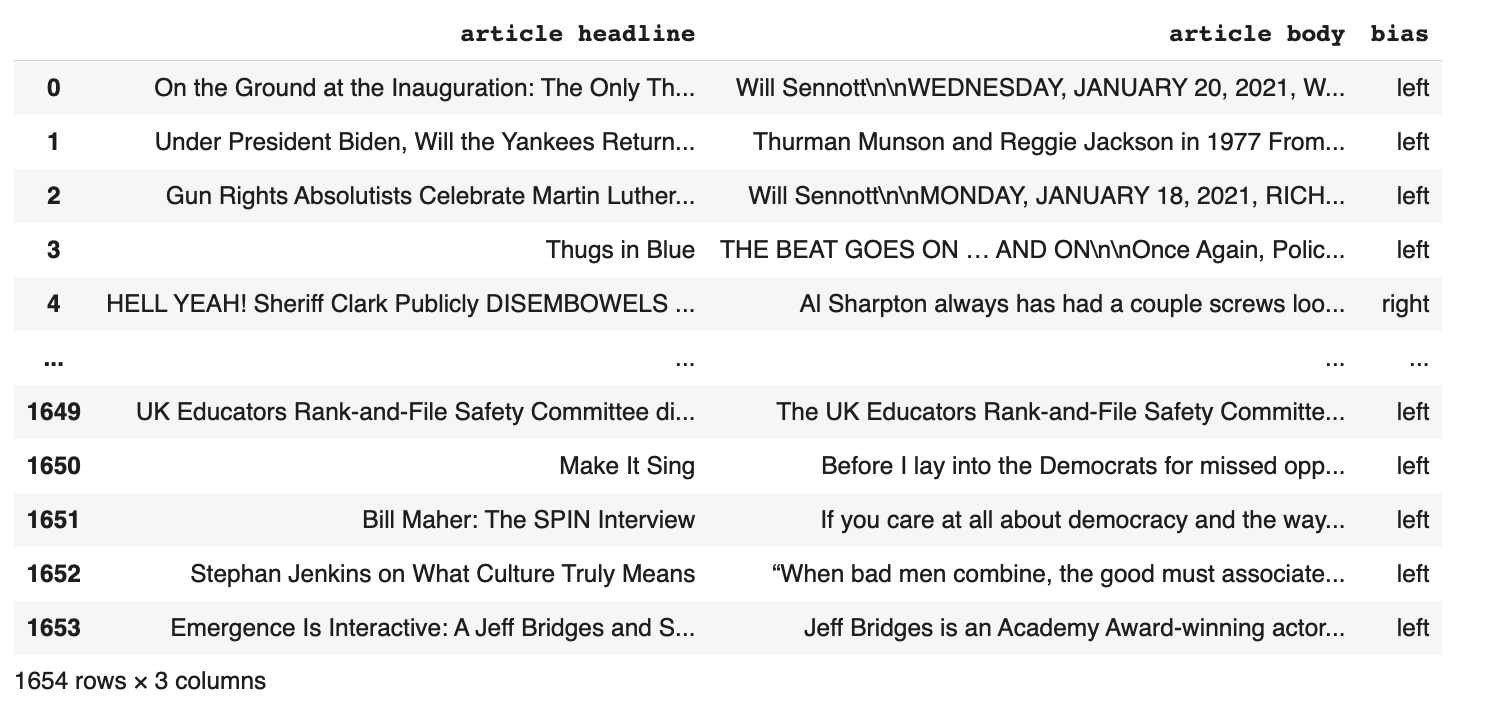
\includegraphics[scale=0.29]{0-img/nmr-bert-data.png}
    \caption{Self-assembled dataset of article headlines, article body text and political affiliation}
    \label{fig:nmr-bert-data}
\end{figure}

\subsection{Data pre-processing}

We pre-process the text by performing lowercasing, punctuation removal, stopword removal and lemmatisation. We opt to keep in exclamation marks and question marks, since BERT can learn features over these to help it detect bias. The Python NLTK \cite{nltk} package is commonly used for stopword removal, however we find it removes words such as `yourselves', `ourselves', `wouldn't', `shouldn't' etc. which could perhaps also be useful for our model. We therefore perform our own more minimalist stopword removal, using mainly basic determiners and prepositions i.e. `I', `you', `in', `at'. Lemmatisation is performed with NLTK's WordNet Lemmatizer \cite{wordnet}.

We encode the labels numerically as \textit{center} := 0, \textit{left} := 1, \textit{right} := 2. We also shuffle the data so that articles from different news sources are spread out in the dataset. The pre-processed dataset is shown in Figure \ref{fig:nmr-bert-data-preprocessed}.

\begin{figure}
    \centering
    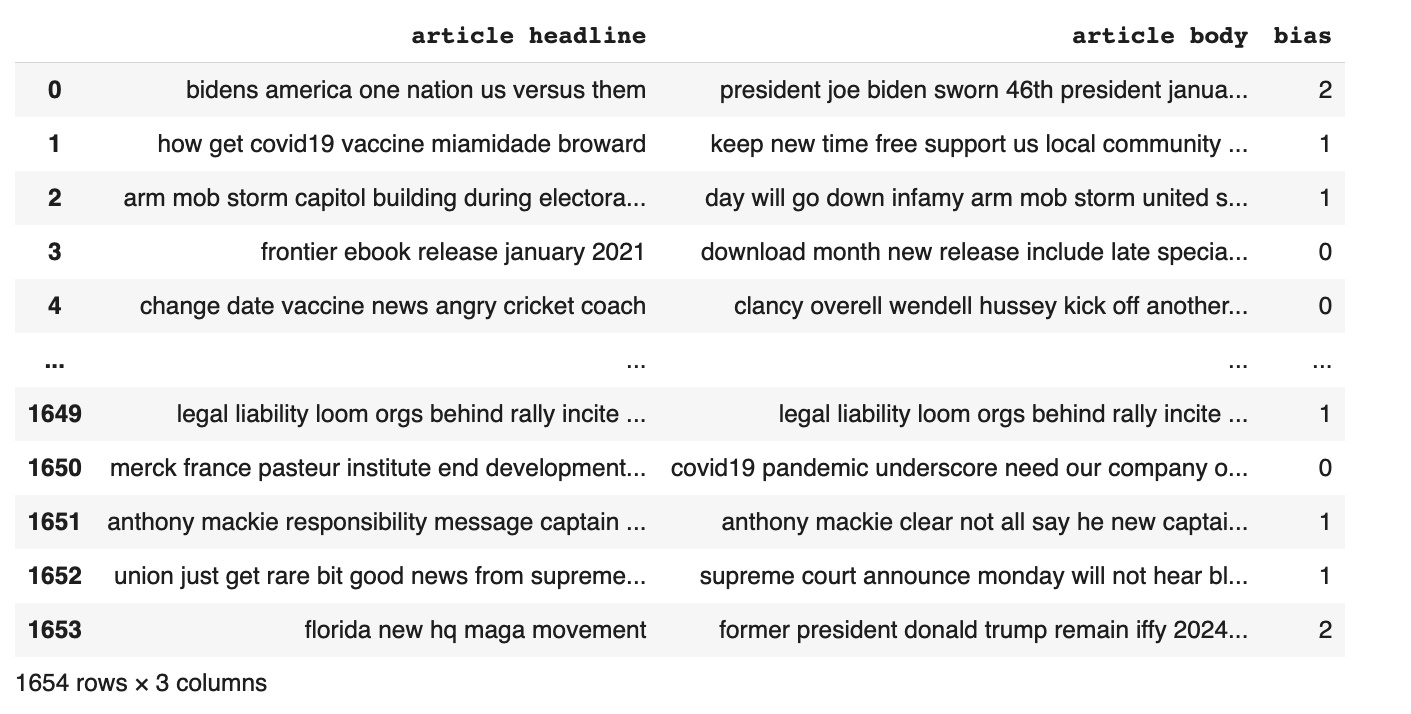
\includegraphics[scale=0.32]{0-img/nmr-bert-data-preprocessed.png}
    \caption{Self-assembled article text dataset after pre-processing}
    \label{fig:nmr-bert-data-preprocessed}
\end{figure}

\subsection{BERT architecture}

Our model is a BERT stack built for sequence classification i.e. with a linear layer at the end and softmax activation to assign a label to the input sequence. We use the pre-trained uncased, base model of BERT since the large model requires too much memory to train with available hardware. We include token IDs, segment IDs and attention masks extracted from the text in our model. A diagram of the model is shown in Figure \ref{fig:bert-sequence-classification}.

BERT only accepts sequences of maximum 512 tokens in length, including the special [CLS] and [SEP] tokens. The maximum headline length with special tokens is 103 tokens, so headlines can be padded up to 512 tokens. However, the maximum article body length is 14,373 tokens, much longer than the limit, so we must truncate article body text to 512 tokens when passing them into BERT.

\subsection{Experimental setup}

We run the BERT sequence classification model using:

\begin{enumerate}
    \item only headlines
    \item only article body text
    \item headlines and body text concatenated together i.e. ``[CLS] \{headline\} [SEP] \{body\}''
\end{enumerate}

Our hypothesis is that using article headlines to predict bias will give higher accuracy than using body text, since headlines distill the essence of the article into just a couple of lines. We also predict using a combined input formed with both headlines and body text will result in higher model accuracy, since more information is being presented to our model.

We use a 70:10:20 train/validation/test split, giving us a training set size of 1157 samples and test set size of 331 samples. We don't use k-fold cross validation with this model due to the small dataset size. With 5 folds each classifier would only be trained with 231 training samples and tested on 66 samples - the training and test sets may not be representative of the overall class distribution.

We use the \texttt{AdamW} \cite{adamw} optimiser, with a learning rate of $ 2 \cdot 10^{-5} $ after hyperparameter tuning. We use a batch size of 10 - we found batches larger than this lead to validation accuracy dropping. We also clip gradient norms to 1 at each training step to prevent any exploding gradients.

\begin{figure}
    \centering
    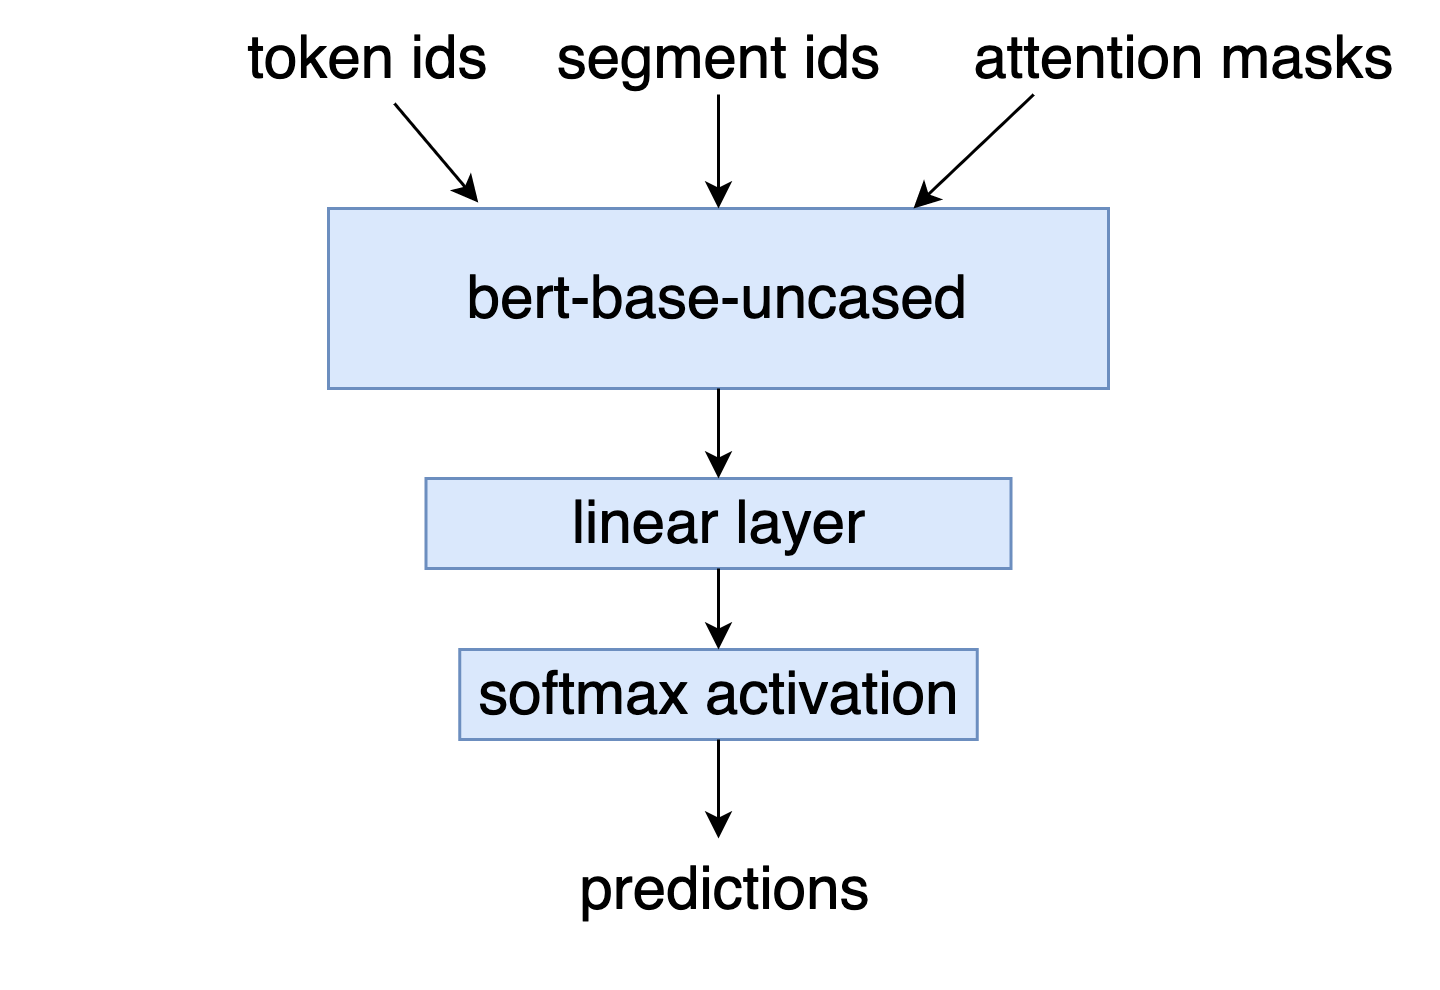
\includegraphics[scale=0.2]{0-img/bert-sequence-classification.png}
    \caption{The BERT sequence classification model}
    \label{fig:bert-sequence-classification}
\end{figure}

\subsection{Evaluation} \label{subsec:nmr-bert-evaluation}

Evaluation metrics comparing the 3 different input types described in the previous section are shown in Figure \ref{fig:nmr-accuracy-f1}.

\todo{compare to earlier classifiers}

\begin{figure}
    \centering
    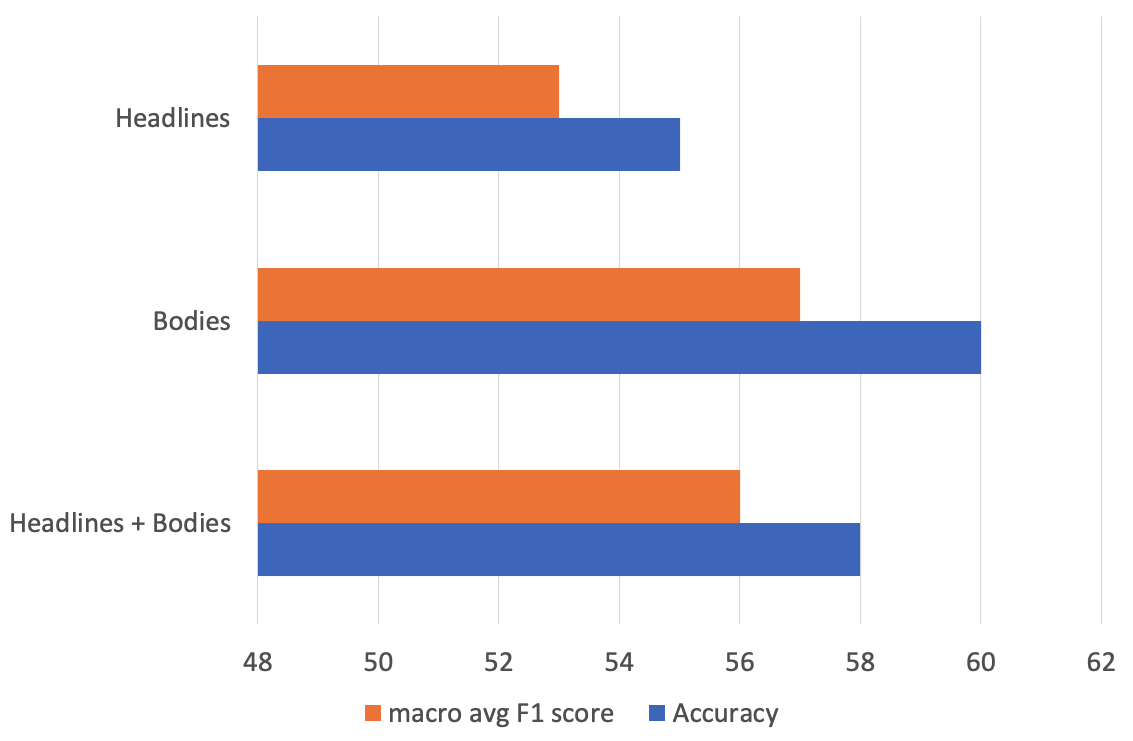
\includegraphics[scale=0.3]{0-img/nmr-accuracy-f1.png}
    \caption{Evaluation metrics for BERT classifier applied to headlines and body text}
    \label{fig:nmr-accuracy-f1}
\end{figure}

We can see using article bodies gives better performance than using article headlines by several percentage points in both accuracy and F1 score, with a highest accuracy of 60\%. Headlines usually distil the content of the article into one or two lines, so this result could be attributed to article bodies simply containing more textual information than headlines (the longest headline in the dataset is only 103 tokens long, much shorter than the maximum 512 tokens allowed).

It's important to note that we have truncated the body text to just the first 512 tokens, and the beginnings of news articles often summarise their main points similar to how a headline would. This could also be why body text gives higher model accuracy than headlines. We explore this further in Section \ref{sec:article-sections} by comparing using the beginning of the article to predict bias vs the middle or the end of the article.

Concatenating headline and body text performs better than simply using headlines, but worse than just using body text. This result is particularly interesting, as our initial hypothesis was that unifying headline and body information would provide the model with more information than using either of the two input types individually. This, however, demonstrates that body text provides more information than any input involving the headlines.

We also explore using RoBERTa for sequence classification, a version of BERT that has been pre-trained further and with more data. Our results are compared in Figure \ref{fig:nmr-roberta-accuracy-f1}. RoBERTa exhibits around the same performance as BERT, with a very minor improvement when using article body text only (61\% accuracy). This demonstrates that further pre-training on the English language does not help the classifier detect bias more easily. 

\begin{figure}
    \centering
    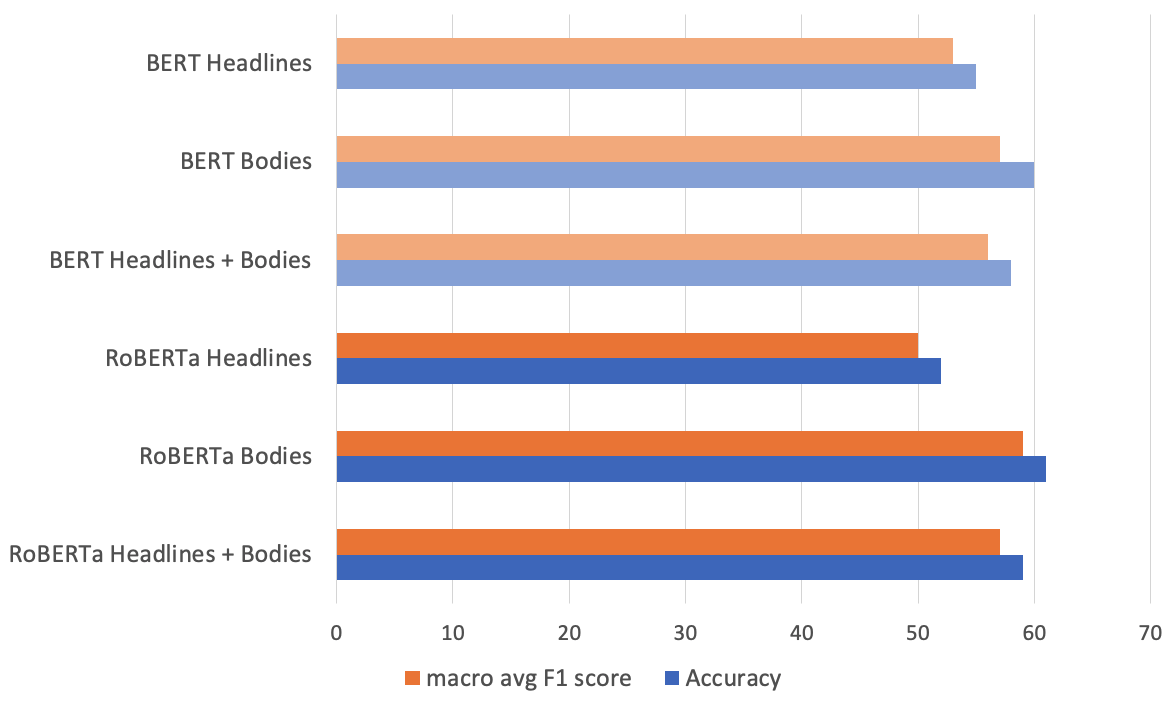
\includegraphics[scale=0.35]{0-img/nmr-roberta-accuracy-f1.png}
    \caption{Evaluation metrics for RoBERTa classifier compared to BERT}
    \label{fig:nmr-roberta-accuracy-f1}
\end{figure}

Chun et al. report an accuracy of 89\% when using BERT to detect political bias in the Russian Troll dataset \cite{russian-troll}, a collection of tweets posted by Russian troll accounts. Our highest accuracy of 61\% is much lower than this. One reason for this discrepancy could be availability of training data - the Russian Troll dataset contains around 3 million tweets, whereas our dataset is very small in comparison, consisting of only 1654 text samples.

Building off the RoBERTa idea, further work could be done examining BERT models pre-trained via predicting bias in text, on top of MLM and NSP, to see if this improves bias detection. We could also explore applying BERT to a much larger dataset - while our self-assembled dataset contains high-quality raw article text, it contains a very small number of text samples compared to other datasets explored in previous literature.

One point to note is that BERT models split tokens up using a subword-level vocabulary, created using the Wordpiece \cite{wordpiece} algorithm. Names therefore get split into subwords after tokenisation, e.g. ``biden'' becomes [`bid', `\#\#en'] and ``covid'' becomes [`co', `\#\#vid']. This could limit the effectiveness of names within the BERT model, since the model will treat the `bid' and `co' tokens just like any other instances of those words in the text. We find that ``biden'' occurs 2,696 times in the dataset, but the `bid' token otherwise only occurs 11 times, so this is not a huge problem in this case. However, ``covid'' occurs 1,201 times in the dataset and the `co' token otherwise occurs another 529 times, which could lead to confusion in the BERT model. Other weaknesses of Wordpiece tokenisation have been explored previously \cite{wordpiece-weaknesses}.

\subsection{Detecting bias from particular article sections} \label{sec:article-sections}

In this section we purely focus on article body text. We want to examine which section of an article (beginning, middle or end) is most helpful to the classifier in determining political bias.

We use the same dataset as in the previous sections. Instead of letting the BERT tokenizer truncate articles to just the first 512 tokens, we isolate 512 tokens from the beginning, middle, and end of article bodies, and pass these into our BERT classification model. Our hypothesis is that using the beginning/end of article text will give higher model accuracy than using text in the middle, since articles often introduce or conclude their main ideas in these sections, and so evidence of political bias will be more evident.

We use the same experimental setup and hyperparameters as in the previous section. Results are shown in Figure \ref{fig:nmr-beginning-middle-end}.

\begin{figure}
    \centering
    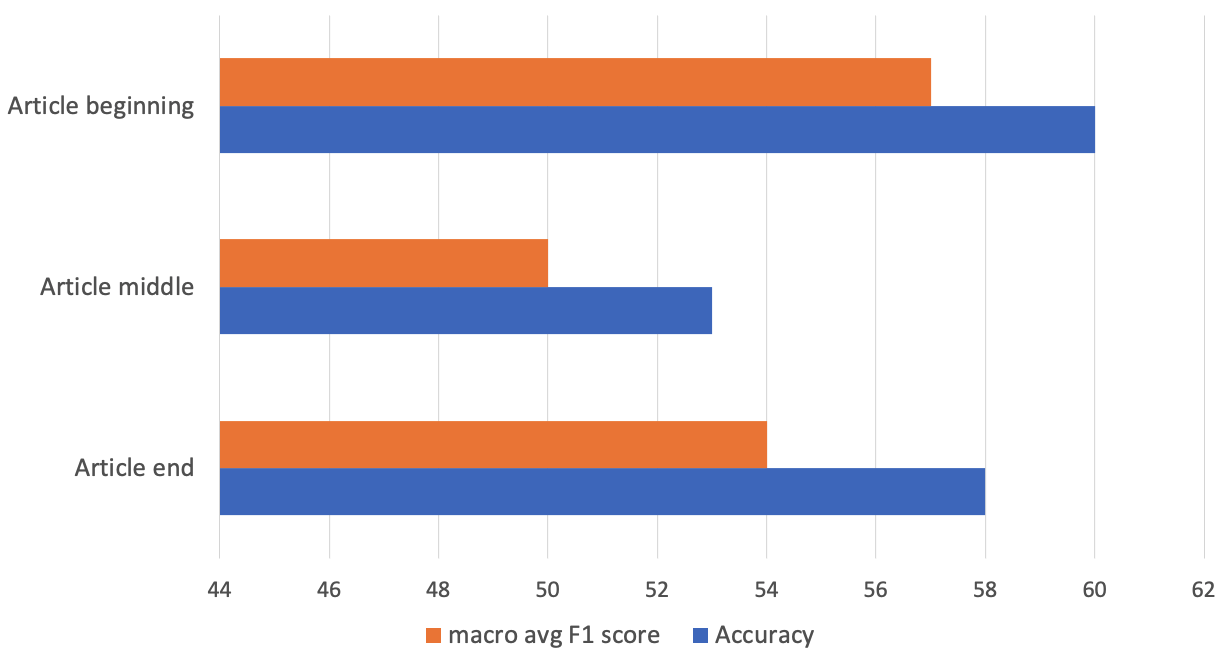
\includegraphics[scale=0.33]{0-img/nmr-beginning-middle-end.png}
    \caption{Evaluation metrics using beginning, middle or end of article text to predict bias}
    \label{fig:nmr-beginning-middle-end}
\end{figure}

We can see our hypothesis has been validated - the model accuracy is better when using text from the beginning or end of an article, rather than from middle sections. Interestingly using introductory text gives a higher accuracy than using concluding text - since introductory text is the first thing the reader sees, perhaps this text is more representative of the overall bias of the article.

The accuracies using the introduction and conclusion of the body text are 60\% and 58\% respectively, however the accuracy we achieved from using article headlines (in the previous section) is 55\%. Therefore, using either the introduction or conclusion of the body text is actually more useful to the classifier than using any headline information at all.